%! Author = domore
%! Date = 8/11/21

\documentclass{amsart}
%\usepackage[margin=1in]{geometry}
\usepackage{afterpage}
\usepackage{tikz}
\usepackage[top=2cm, bottom=2cm, outer=0cm, inner=0cm]{geometry}
\usepackage{graphicx}
\usepackage{xcolor}
\usepackage{color}
\usetikzlibrary{fadings}
\usepackage[absolute,overlay]{textpos}
% https://tex.stackexchange.com/questions/167719/how-to-use-background-image-in-latex

\begin{document}

\DeclareFixedFont{\titlefont}{T1}{ppl}{b}{}{0.4in}
\DeclareFixedFont{\subtitlefont}{T1}{ppl}{b}{}{0.15in}
\afterpage{\restoregeometry}
\newgeometry{left=1in, right=1in,top=1in, bottom=0in}
\definecolor{mytan}{HTML}{FF6515}
\pagecolor{mytan}\afterpage{\nopagecolor}

%\thispagestyle{empty}
{\color{white}
\begin{flushright}
\titlefont Wine Quality\\
\subtitlefont Francisco Prado Moreno, Vienna 2021
\end{flushright}
%\vfill
}

\tikz[remember picture,overlay] \node[scope fading=north, inner sep=0pt, outer sep=0pt] at (current page.center){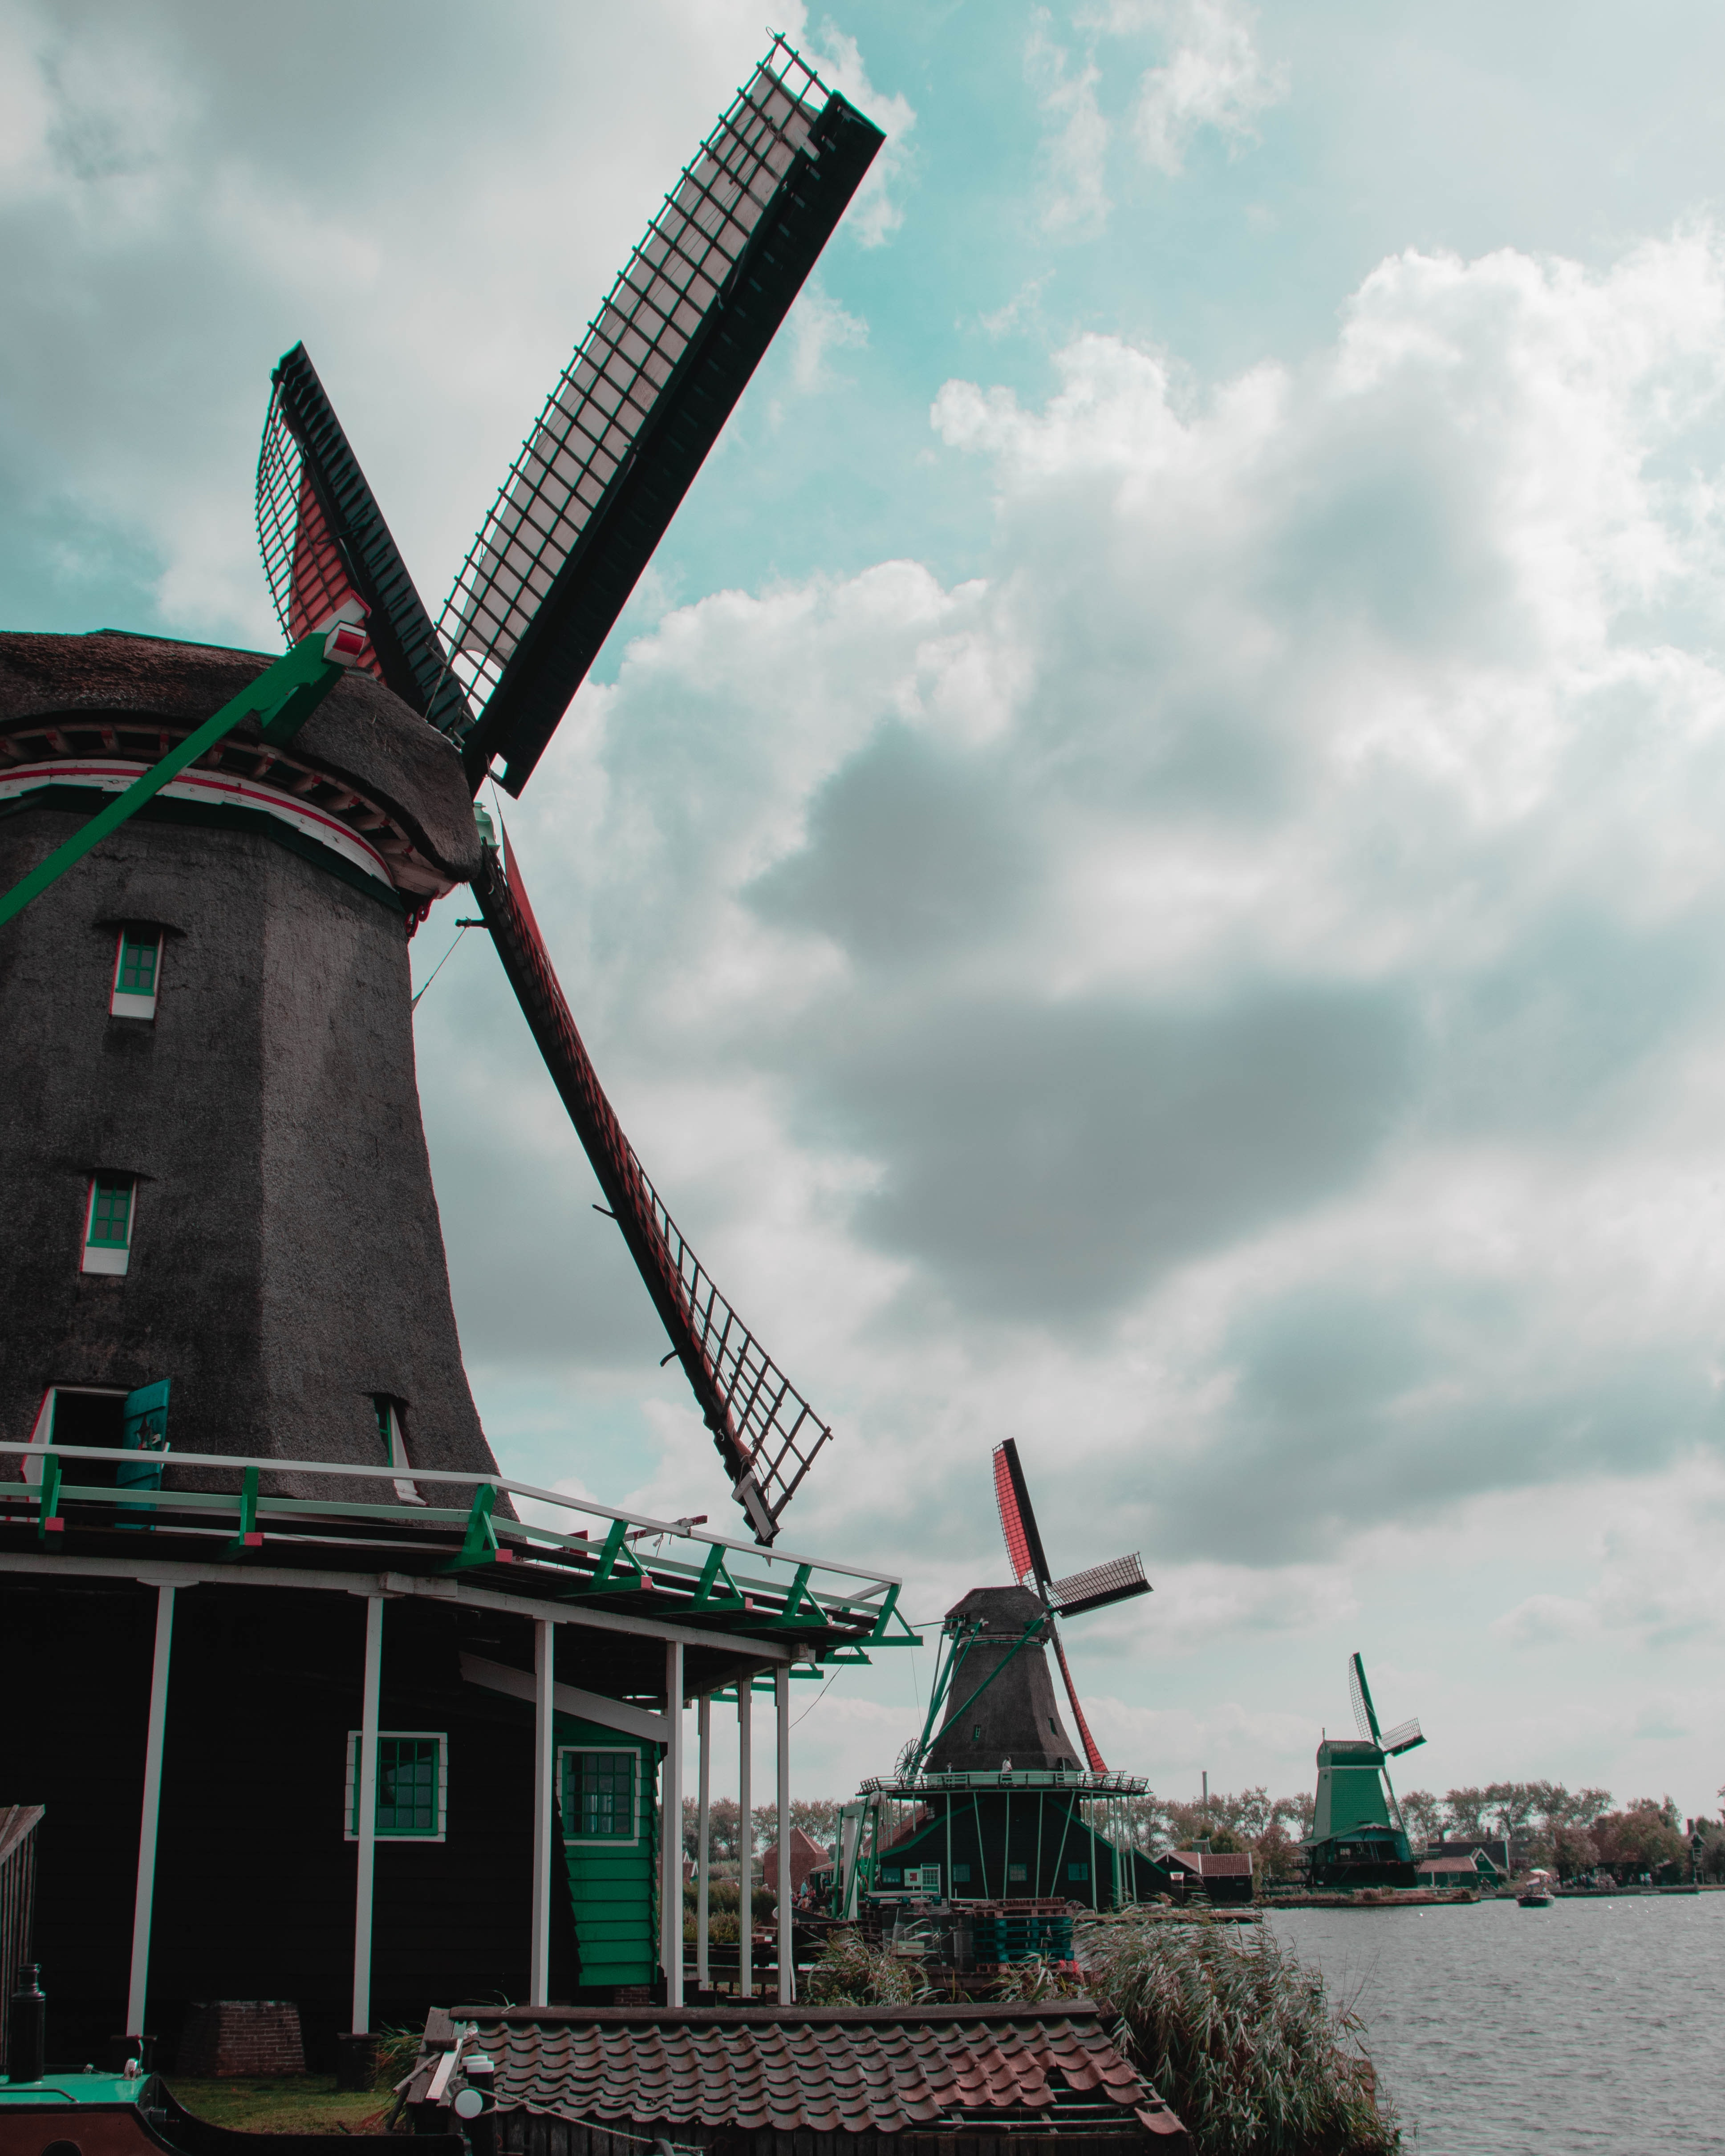
\includegraphics[width=\paperwidth,height=\paperheight]{figs/mill_amsterdam.jpg}};
\newpage
%\clearpage

\thispagestyle{empty}


\begin{flushright}
\titlefont Wine Quality\\
\subtitlefont Francisco Prado Moreno, Vienna 2021
\end{flushright}
%\vfill

\tikz[remember picture,overlay] \node[opacity=0.3,inner sep=0pt] at (current page.center){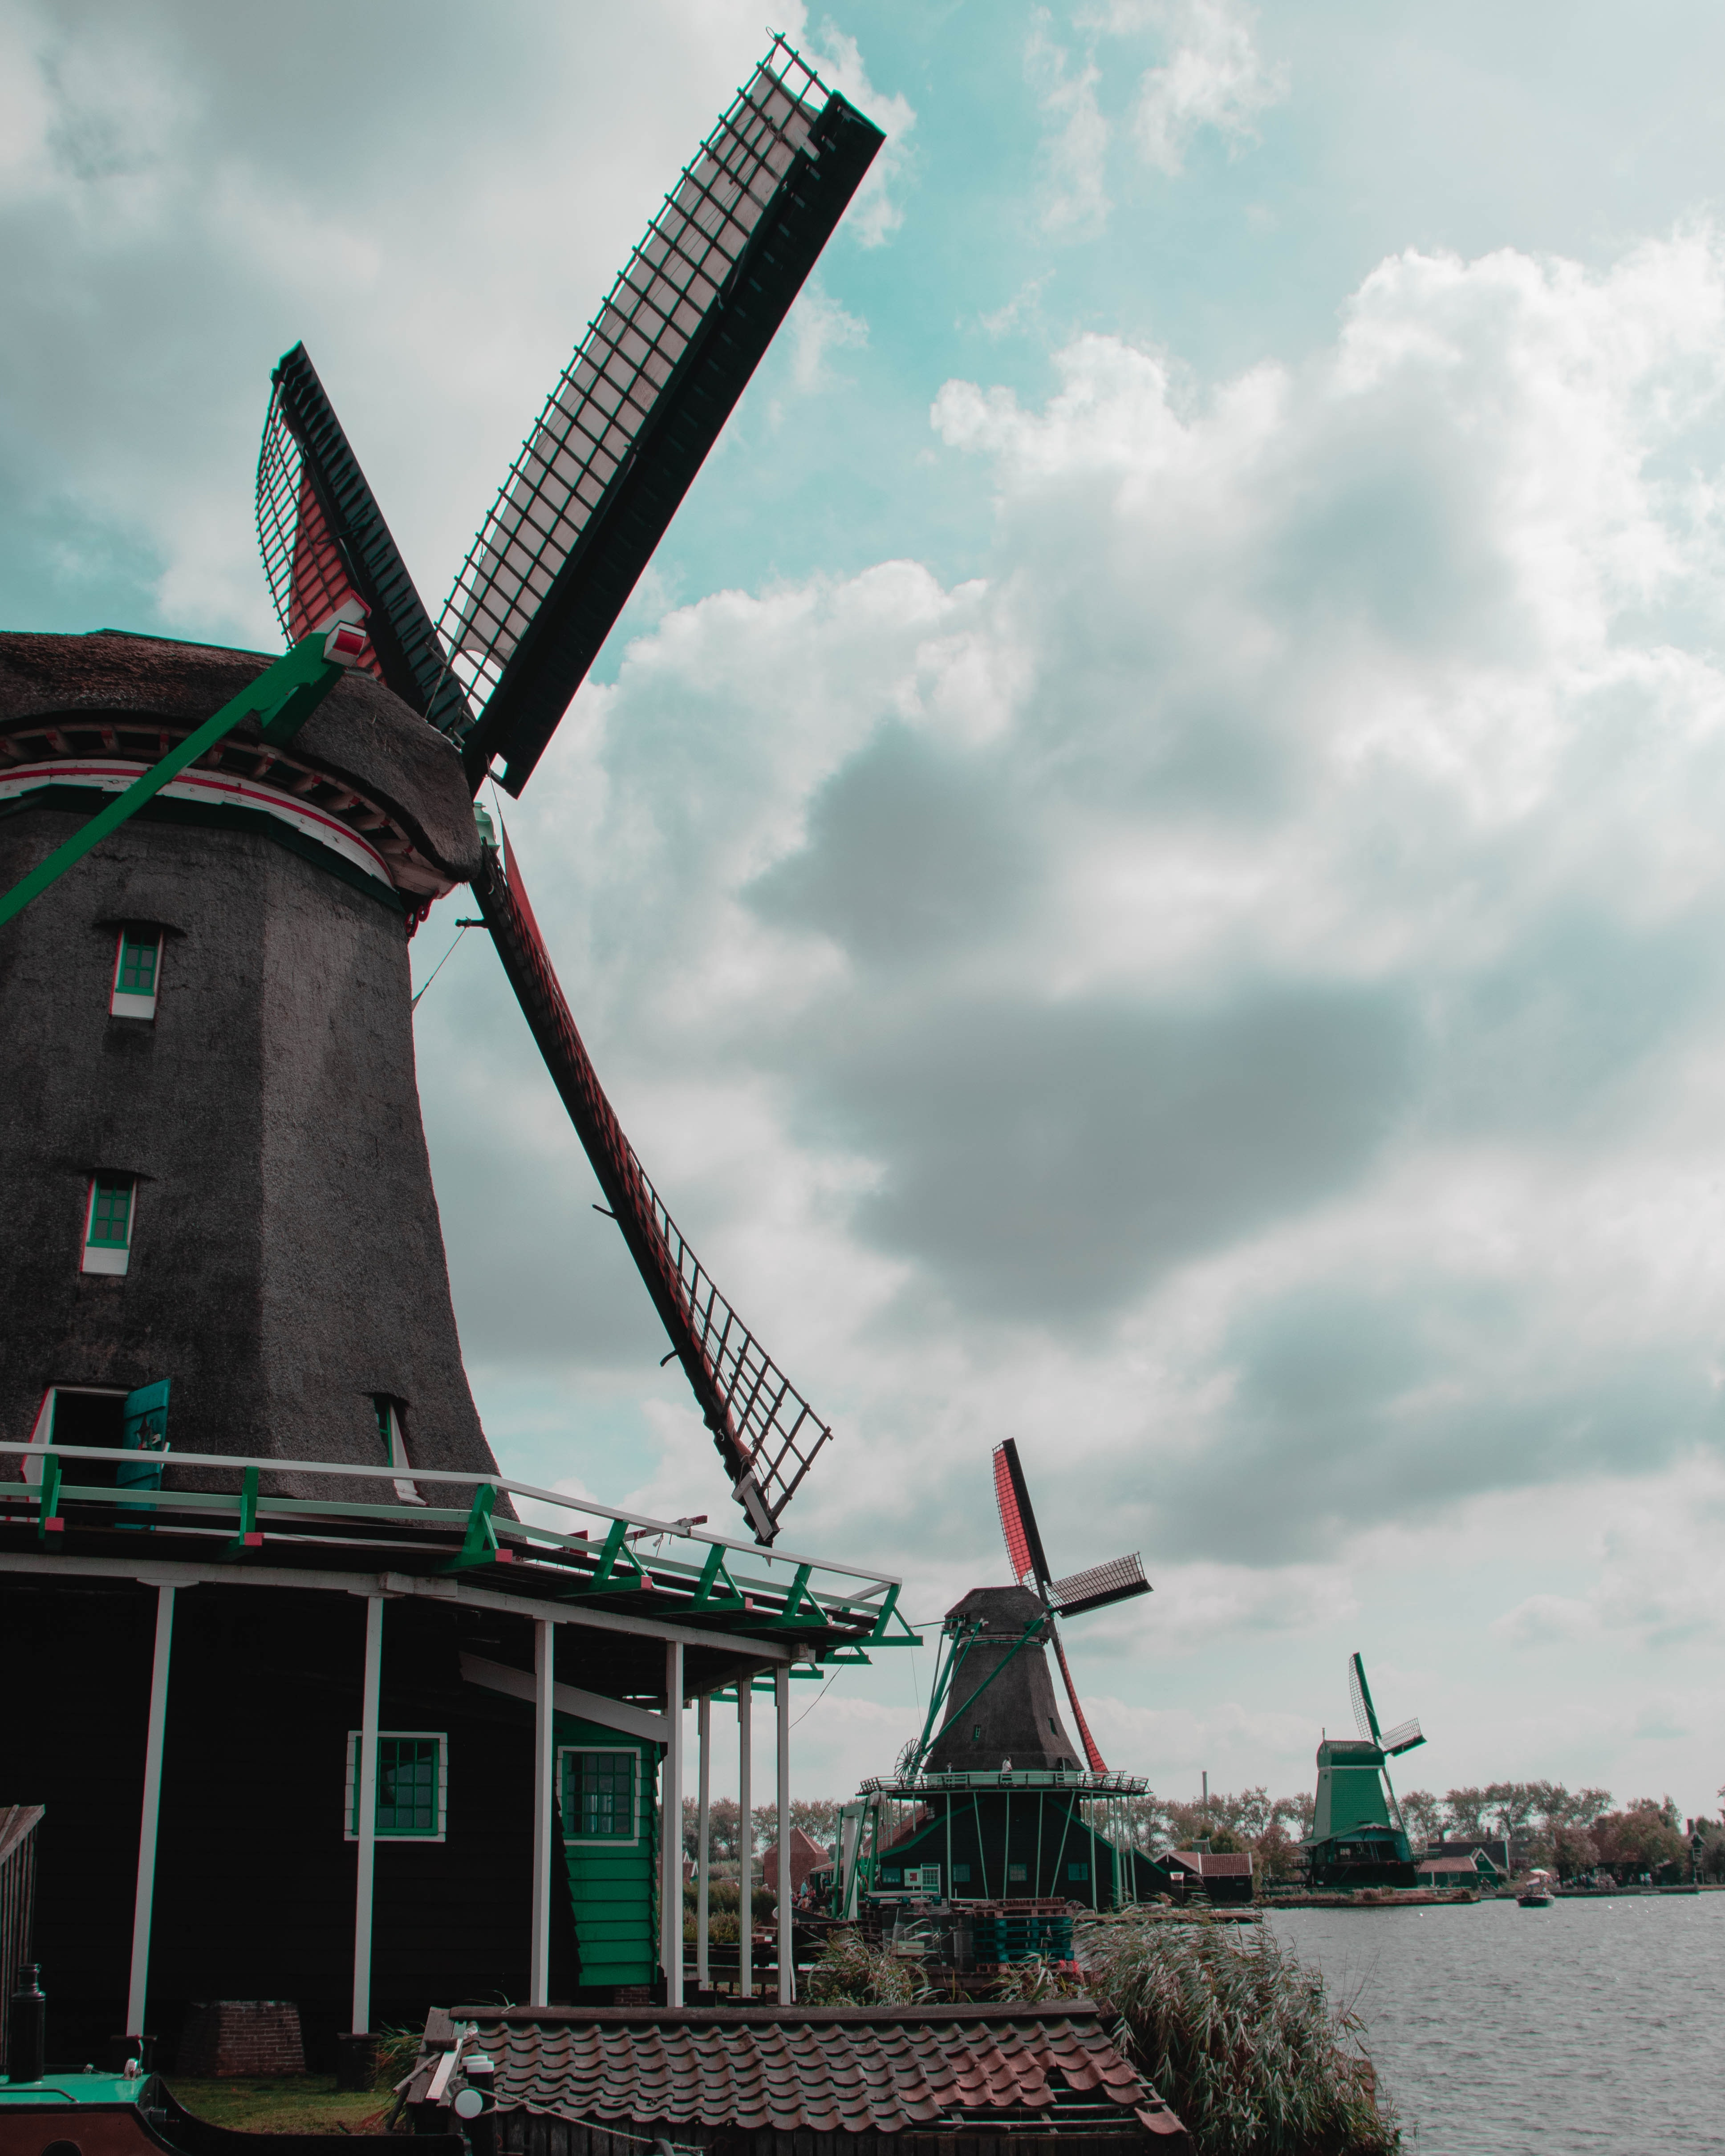
\includegraphics[width=\paperwidth,height=\paperheight]{figs/mill_amsterdam.jpg}};
\clearpage
% \tikz[remember picture,overlay] \node[opacity=0.3,inner sep=0pt] at (current page.center){\includegraphics[width=\paperwidth,height=\paperheight]{example-image}};
%\clearpage
% for additional pages after the title, uncomment the following line first:
% \clearpage


\begin{flushright}
\titlefont Wine Quality\\
\subtitlefont Francisco Prado Moreno, Vienna 2021
\end{flushright}
%\vfill

\tikz[remember picture,overlay] \node[opacity=0.3,inner sep=0pt] at (current page.center){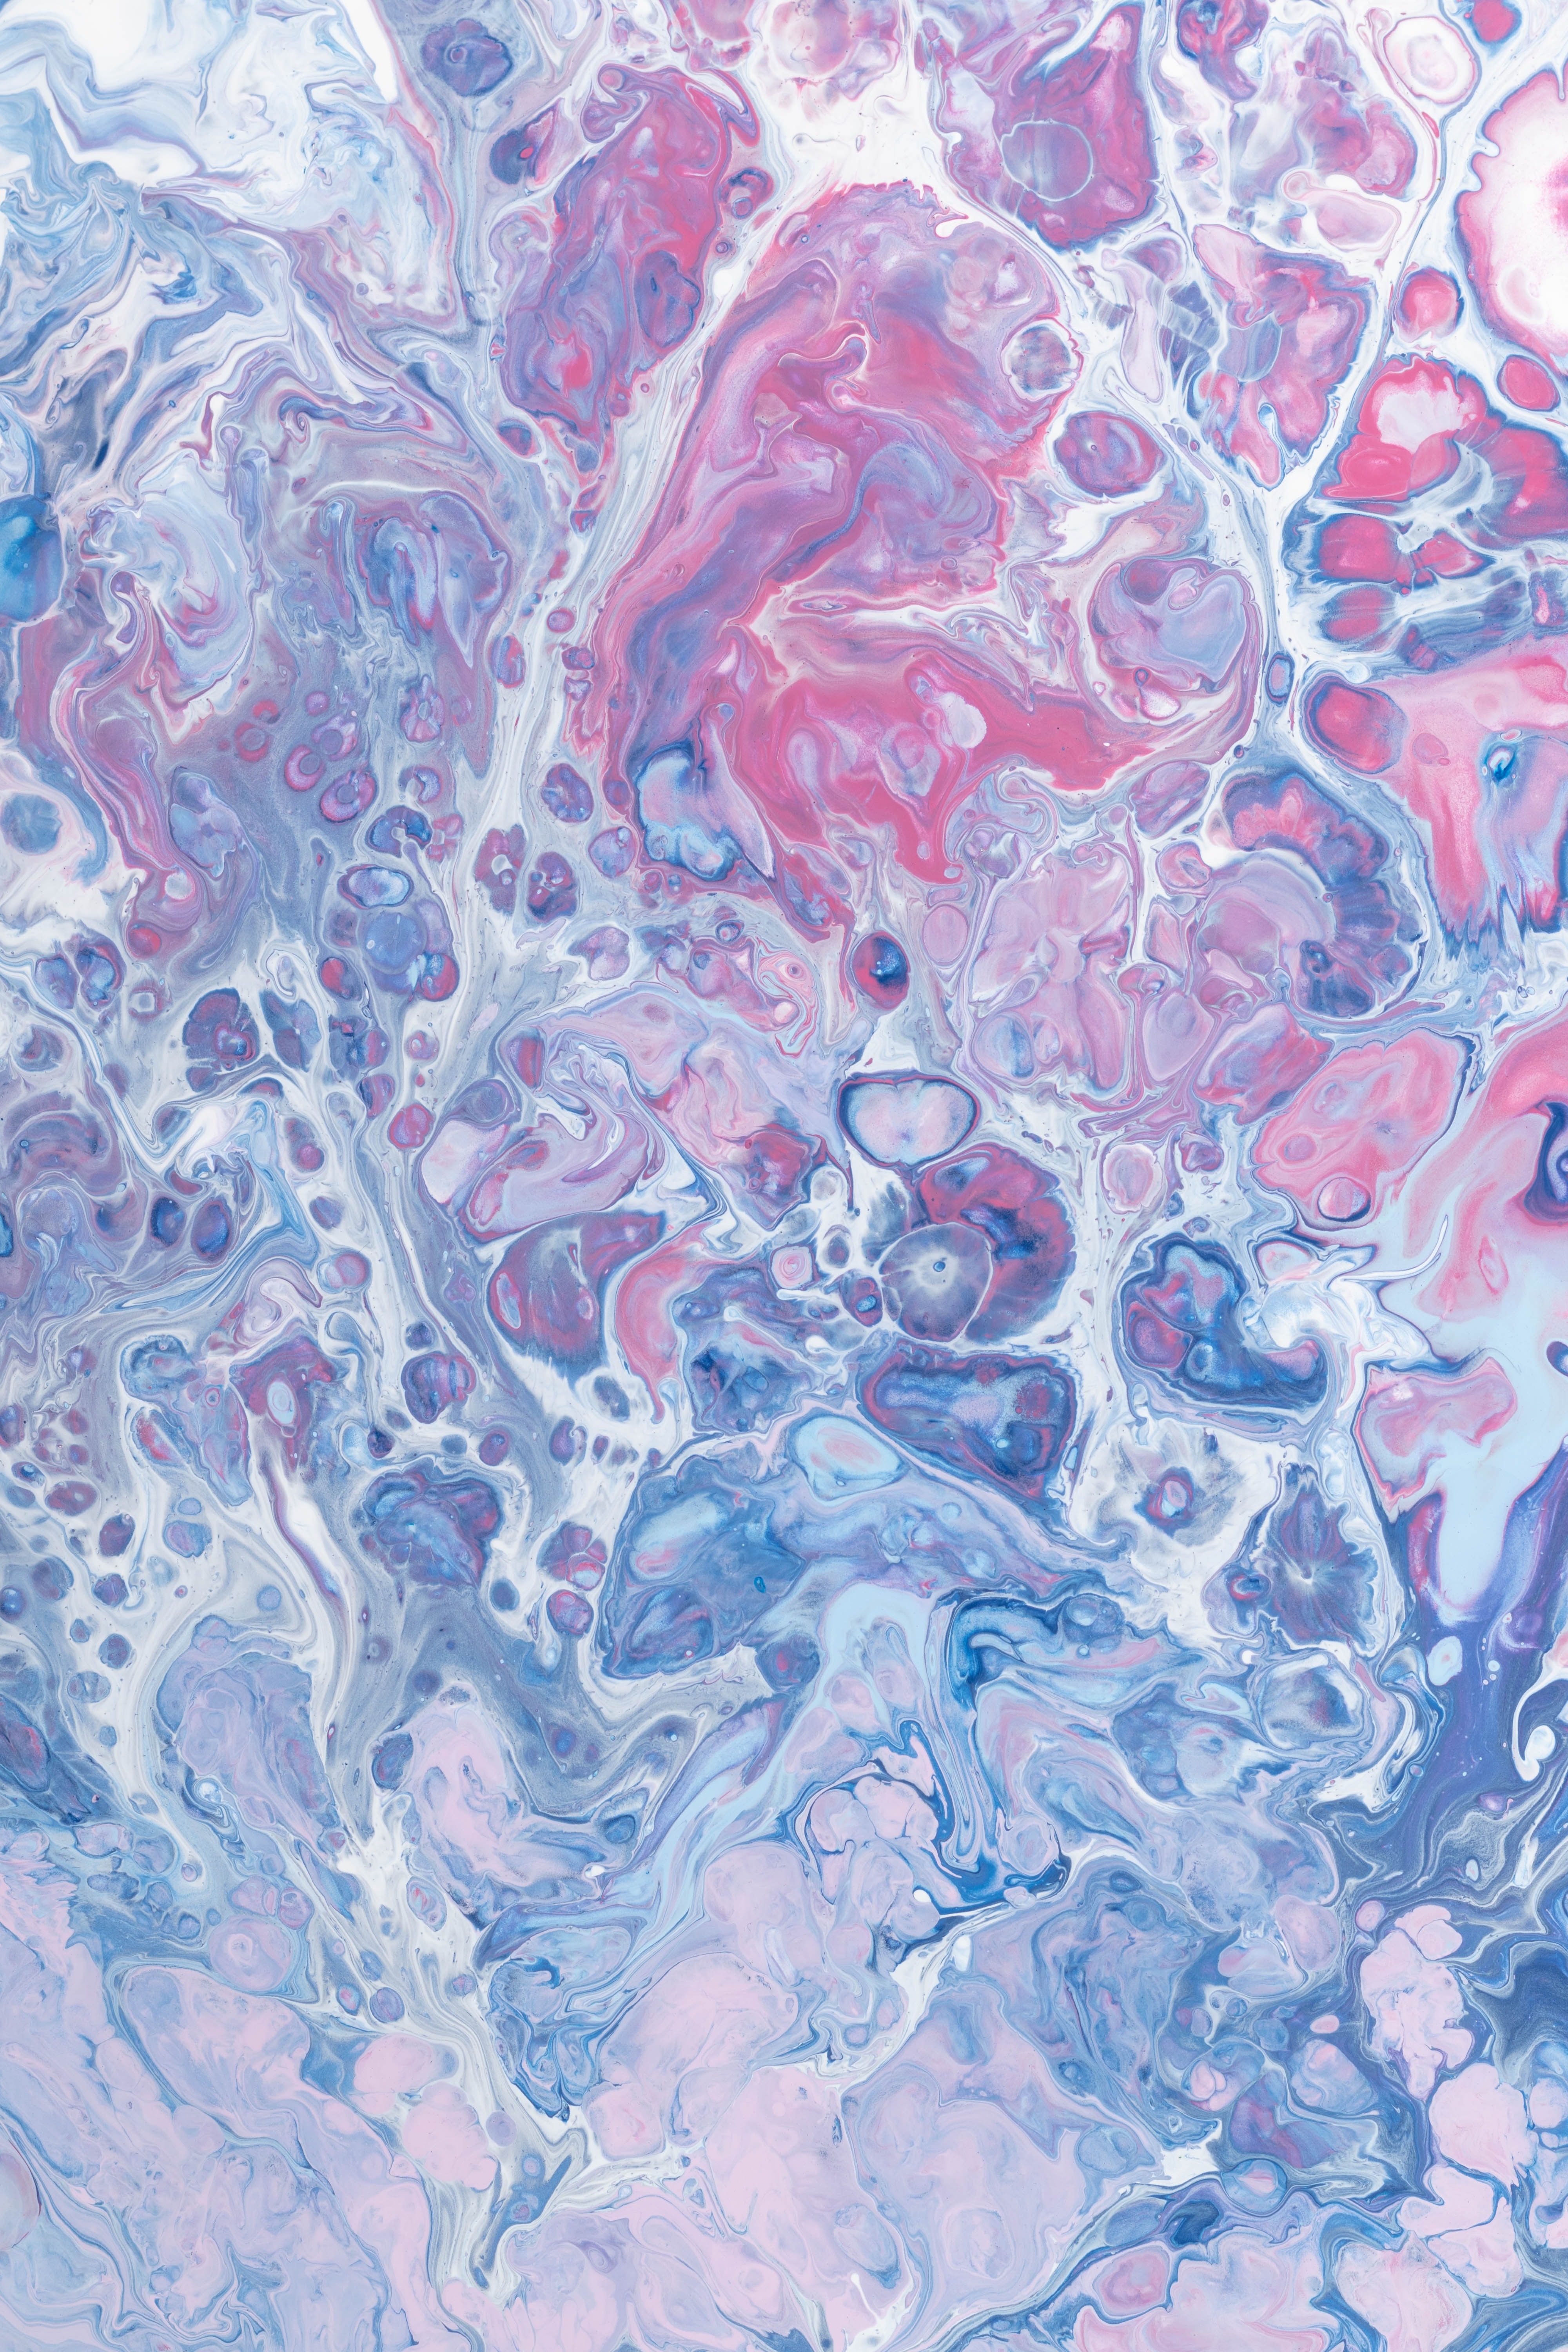
\includegraphics[width=\paperwidth,height=\paperheight]{figs/patterns.jpg}};
\clearpage

\begin{flushright}
\titlefont Wine Quality\\
\subtitlefont Francisco Prado Moreno, Vienna 2021
\end{flushright}
%\vfill

%\begin{textblock*}{10cm}(9cm,20cm) % {block width} (coords)
%\begin{flushright}
%\titlefont Wine Quality\\
%\subtitlefont Francisco Prado Moreno, Vienna 2021
%\end{flushright}
%\end{textblock*}

\tikz[remember picture,overlay] \node[opacity=0.3,inner sep=0pt] at (current page.center){
\includegraphics[width=\paperwidth,height=\paperheight]{figs/shapes.jpg}};

%{\textblockcolour{white}
%\begin{textblock*}{10cm}(9cm,20cm) % {block width} (coords)
%hhgdhasdkjashdkjhasddasjhdjkashdkhkjsdhkasjhdkjashkdjhaskjdhksjadhkasjhdkjashdkjasdhkjash\\
%    fdsfhsdjkf
%    \vspace{1cm}
%    diasdljaskldjkasjdlkjsalkjd
%\end{textblock*}}
\clearpage


\begin{flushright}
\titlefont Wine Quality\\
\subtitlefont Francisco Prado Moreno, Vienna 2021
\end{flushright}
%\vfill

\tikz[remember picture,overlay] \node[opacity=0.6,inner sep=0pt] at (current page.center){
\includegraphics[width=\paperwidth,height=\paperheight]{figs/abstract.jpg}};
\clearpage


\end{document}